\begin{figure*}[htb!]
	\begin{center}
		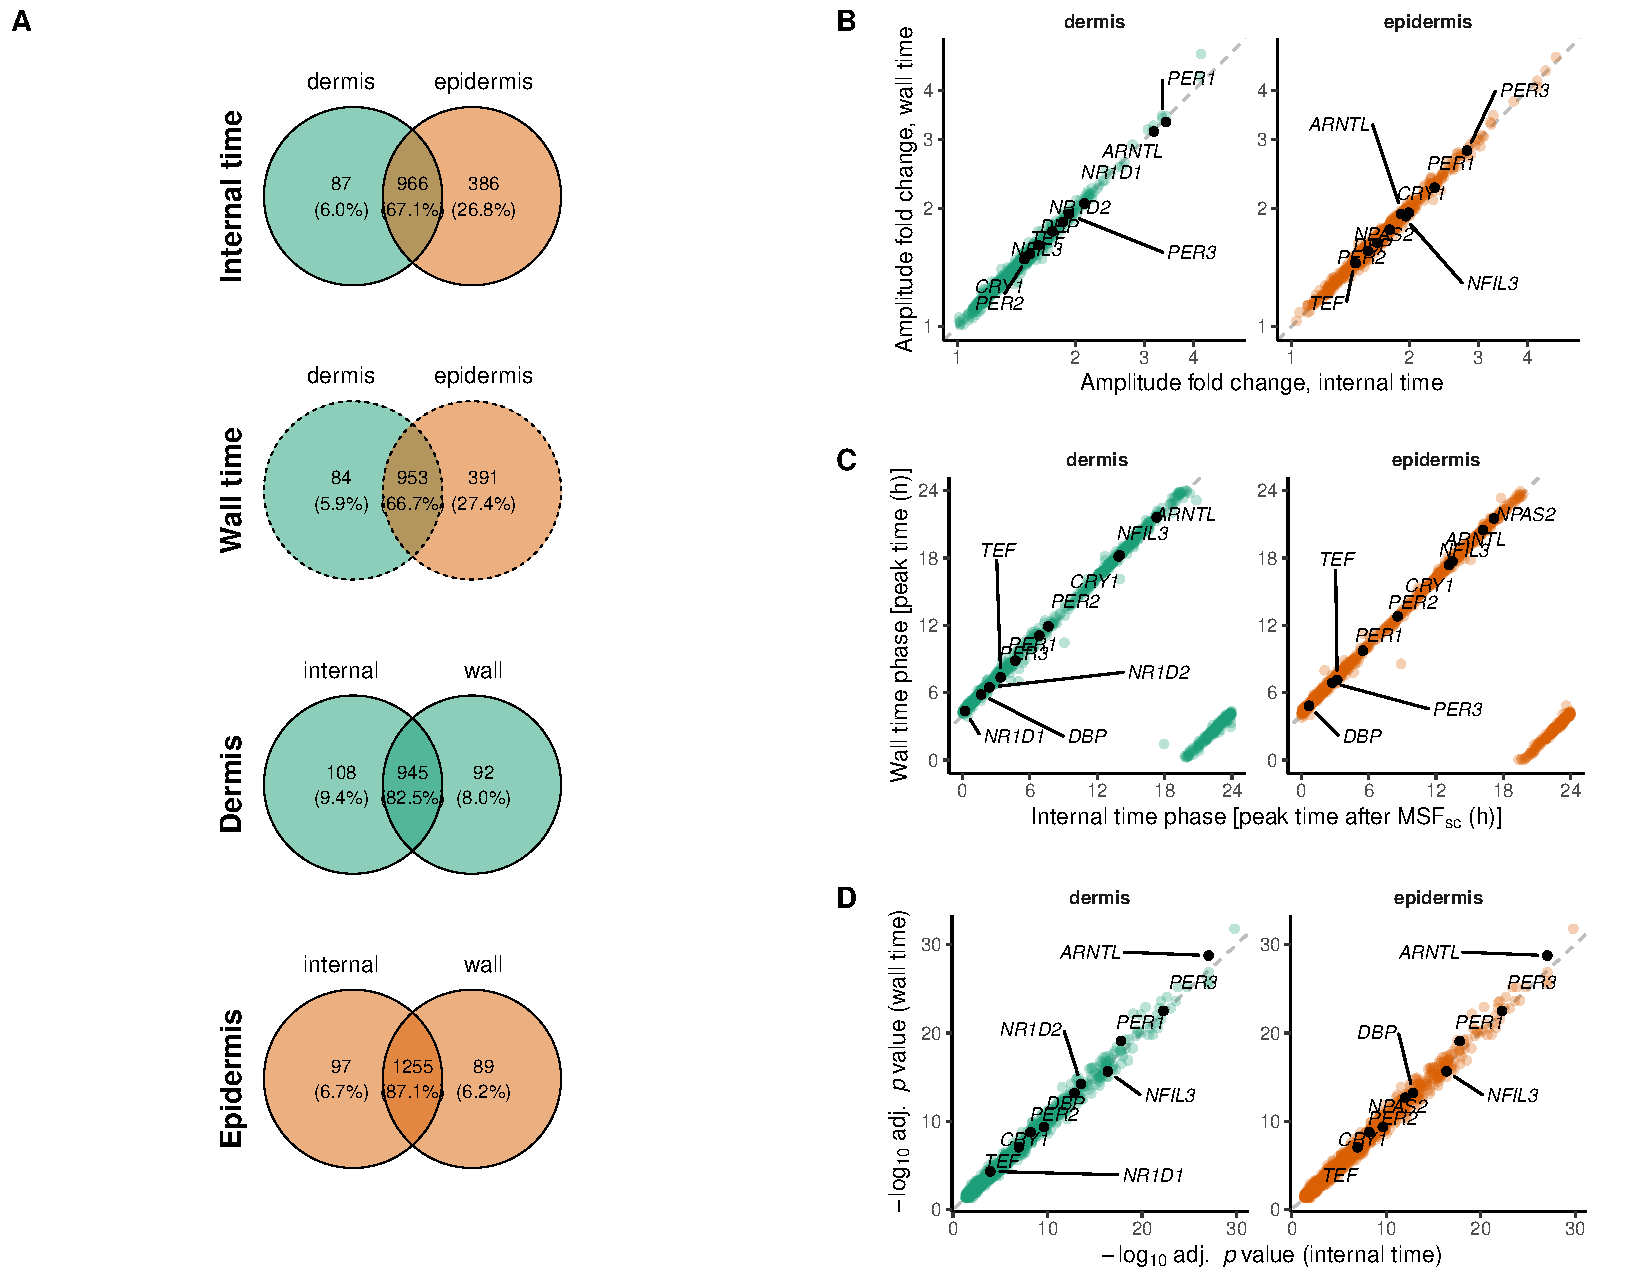
\includegraphics[scale=0.55]{./Figures/suppfig1.pdf}
		\caption{\textbf{Analysis of the circadian transcriptome in human dermis and epiderms done with external (instead of internal) time.} \textbf{A.} Venn diagram visualization of the number of genes identified as circadian in dermis (green) vs. epidermis (orange) and in the analysis using internal time (solid line) or wall time (dashed line). \textbf{B.} Amplitude correlation of genes identified as rhythmic with the internal time analysis compared to external time analysis. \textbf{C.} Acrophase correlation of genes identified as rhythmic with the internal time analysis compared to external time analysis. \textbf{D. }BH-adjusted \textit{p} value correlation of rhythmic genes identified with internal vs. external time analysis. \\
		% \textcolor{red}{Also to the question of whether genes with higher amplitude in internal time analysis are related to some specific functions, see noter on 9.9.21, nothing too interesting. inkscape: wall time in dashed}
	}
		\label{fig:suppfig1}
	\end{center}
\end{figure*}
\clearpage

%----------------------------------------------------------------------------------------
%----------------------------------------------------------------------------------------

\begin{figure*}[h!tb]
	\begin{center}
		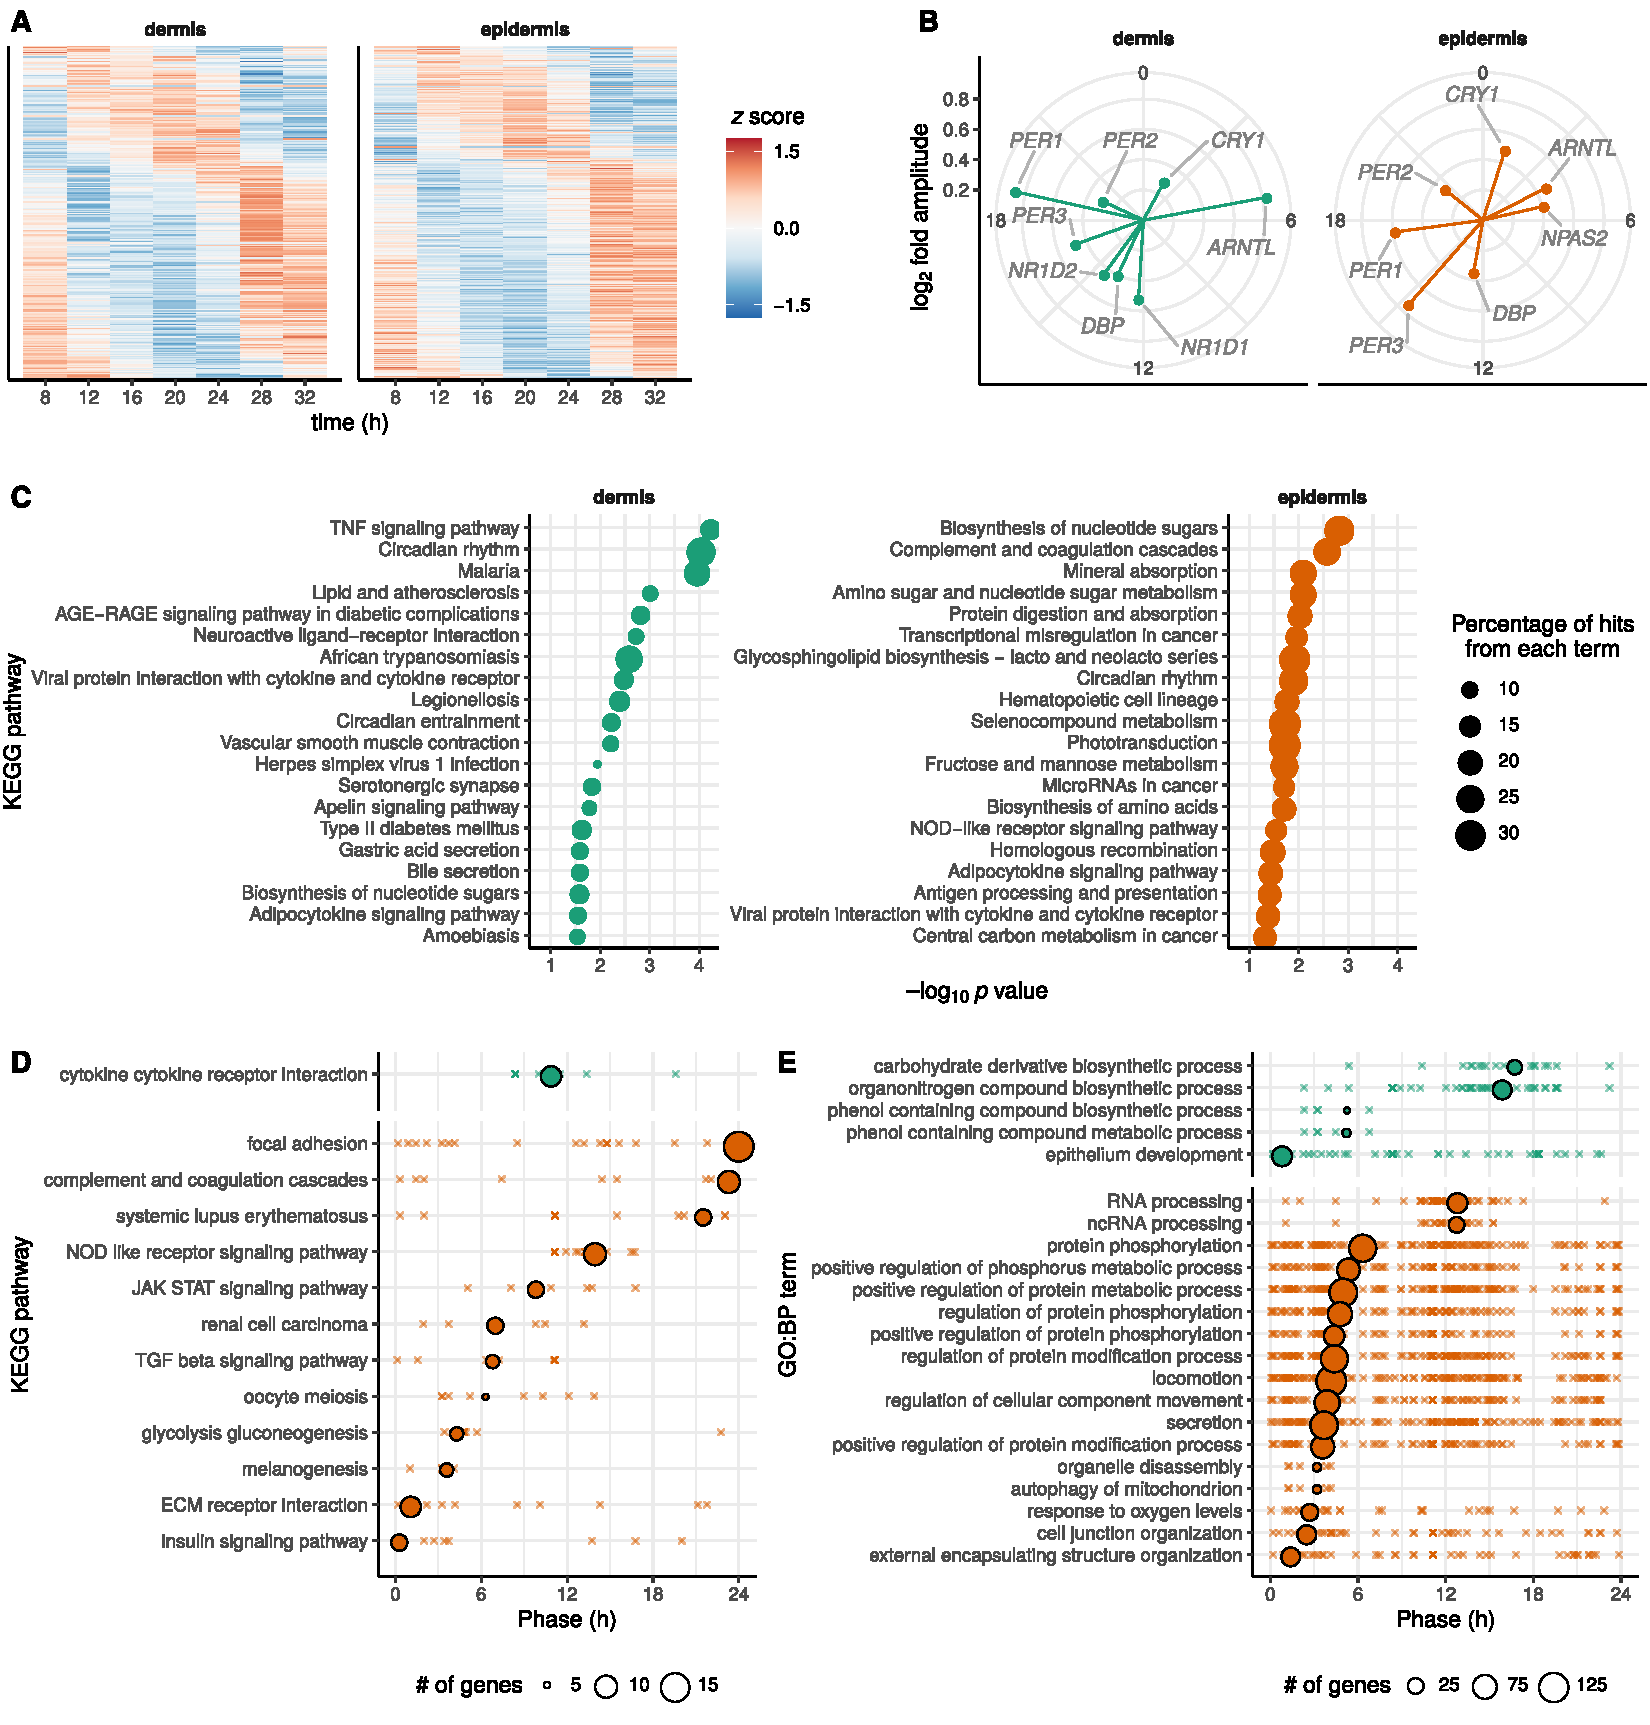
\includegraphics[scale=0.55]{./Figures/suppfig2.pdf}
		%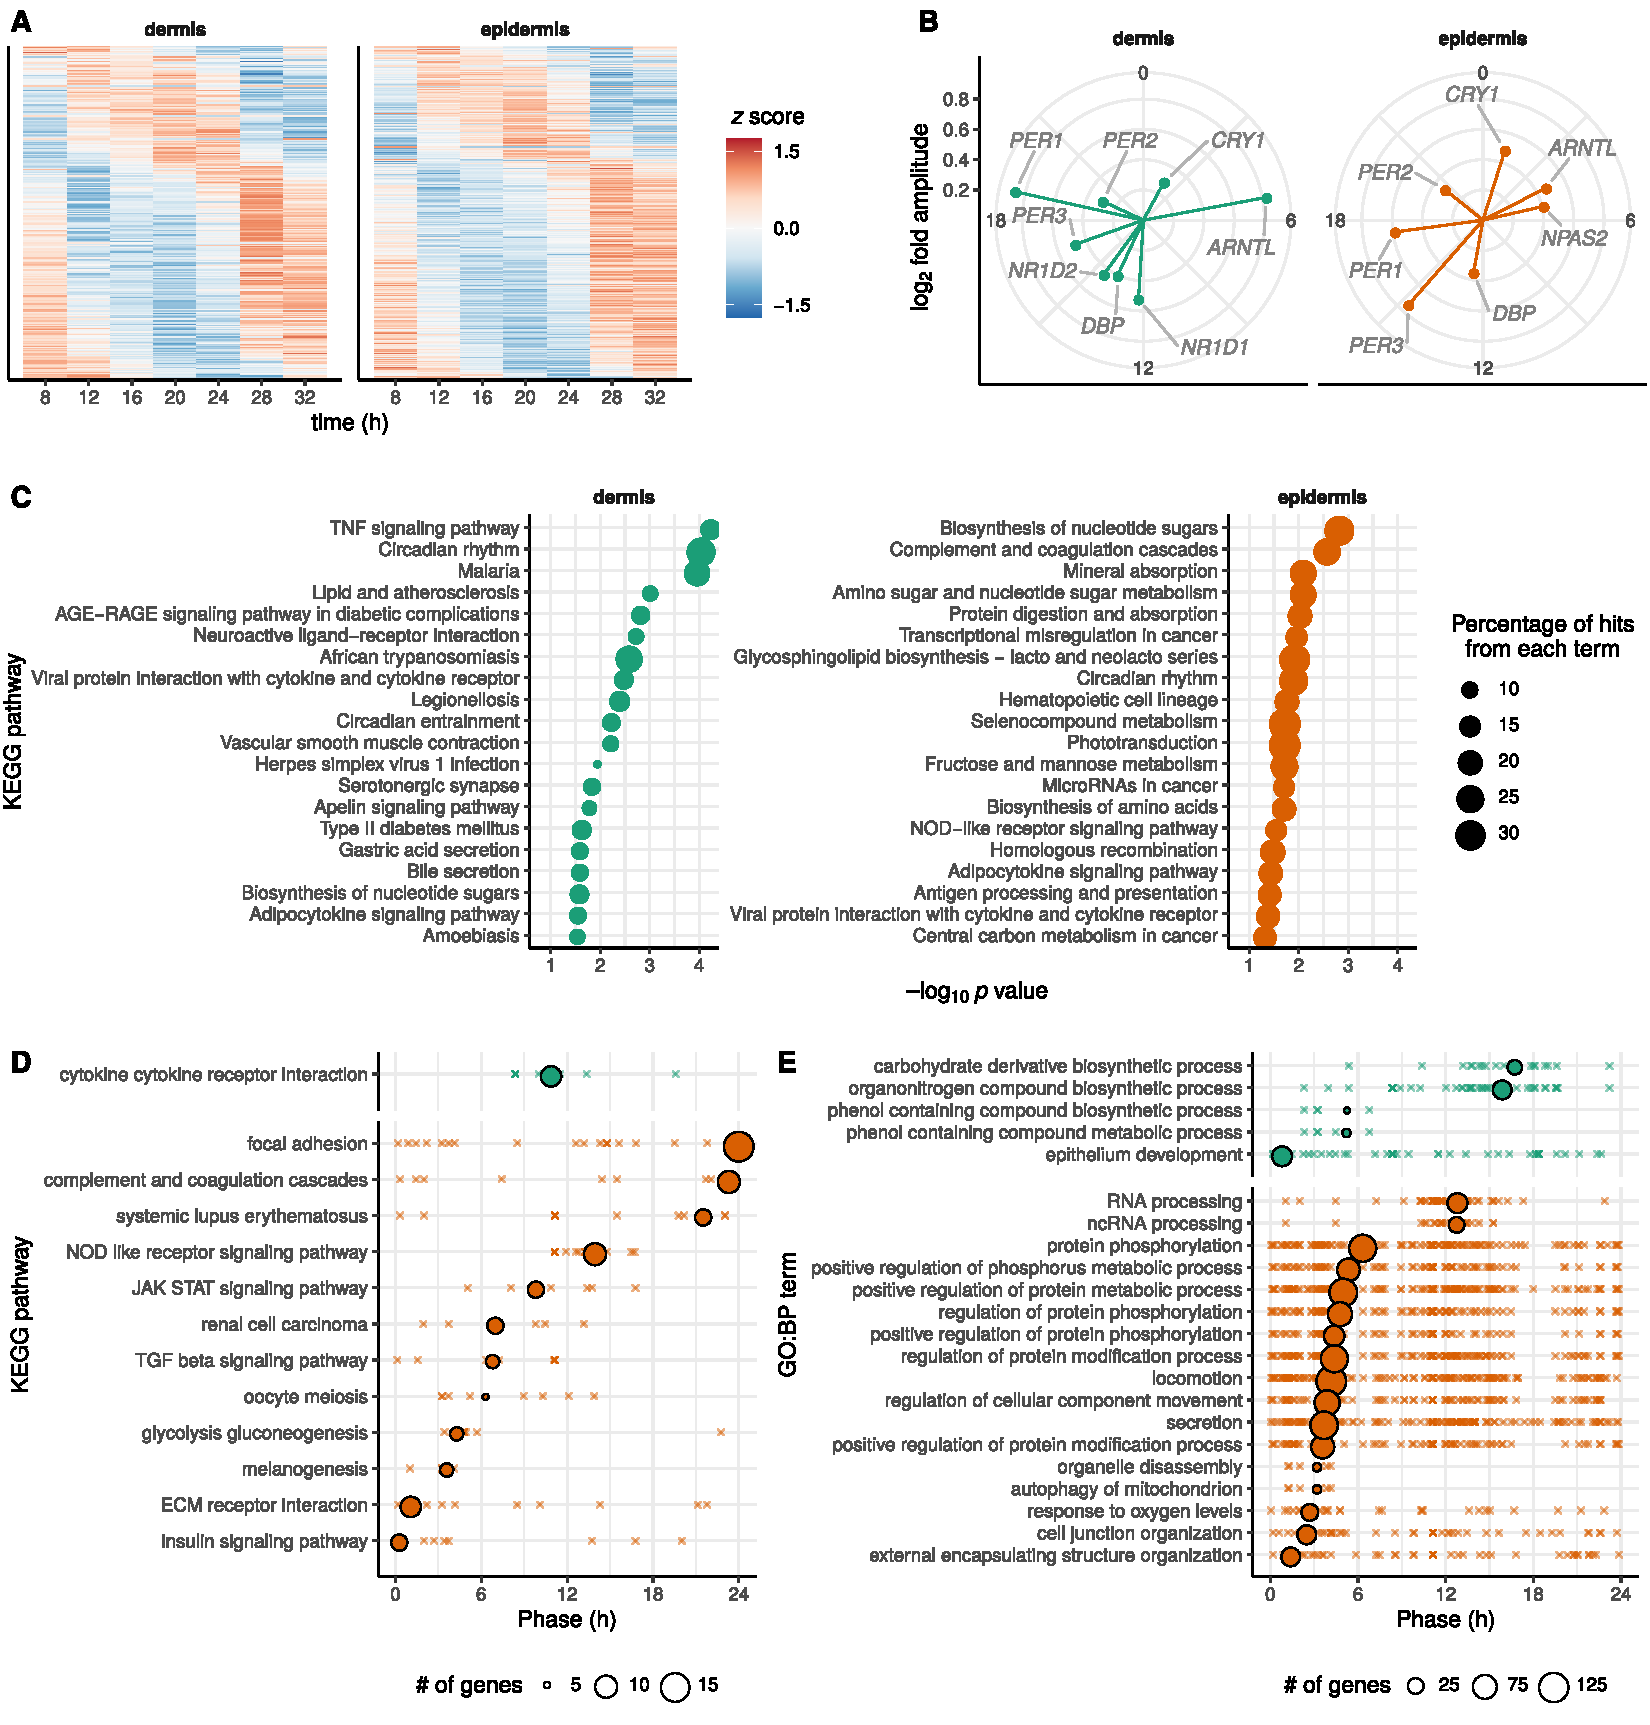
\includegraphics[scale=0.55]{./Figures/suppfig2.pdf}
		\caption{\textbf{Analysis of the human circadian transcriptome in dermis and epiderms with respect to internal time.} Acrophases and amplitudes of rhythmic genes were estimated from the cosinor analysis at FDR$<0.05$ and relative ampitude $>0.26$. \textbf{A.} $z$ score-normalized, acrophase-ordered expression heatmap of the circadian transcriptome components from human dermis (left) and epidermis (right).\textbf{ B.} Expression profiles of circadian core clock genes in human dermis (left) and epidermis (right). Arrow direction represents phase (expressed in units of circadian \textit{internal} time) and arrow length depicts amplitude. \textbf{C. }Circadian KEGG pathway enrichment analysis of the rhythmic genes in dermis (green) and epidermis (orange). The top 20 enriched pathways (with a minimum gene set of 5 terms per category) in each layer are shown. \textbf{D.} Summary of significantly phase-clustered circadian GO terms ($q<0.05$) and KEGG pathways ($q<0.25$) in dermis (green) and epidermis (orange) as determined by PSEA. Sets containing fewer than five circadian transcripts were excluded from the analysis. }%Heatmaps of Spearman correlation (rho) between each pair of core-clock genes for human dermis and epidermis. q < 0·01}
		\label{fig:suppfig2}
	\end{center}
\end{figure*}

%----------------------------------------------------------------------------------------
%----------------------------------------------------------------------------------------

\begin{figure*}[h!tb]
	\begin{center}
		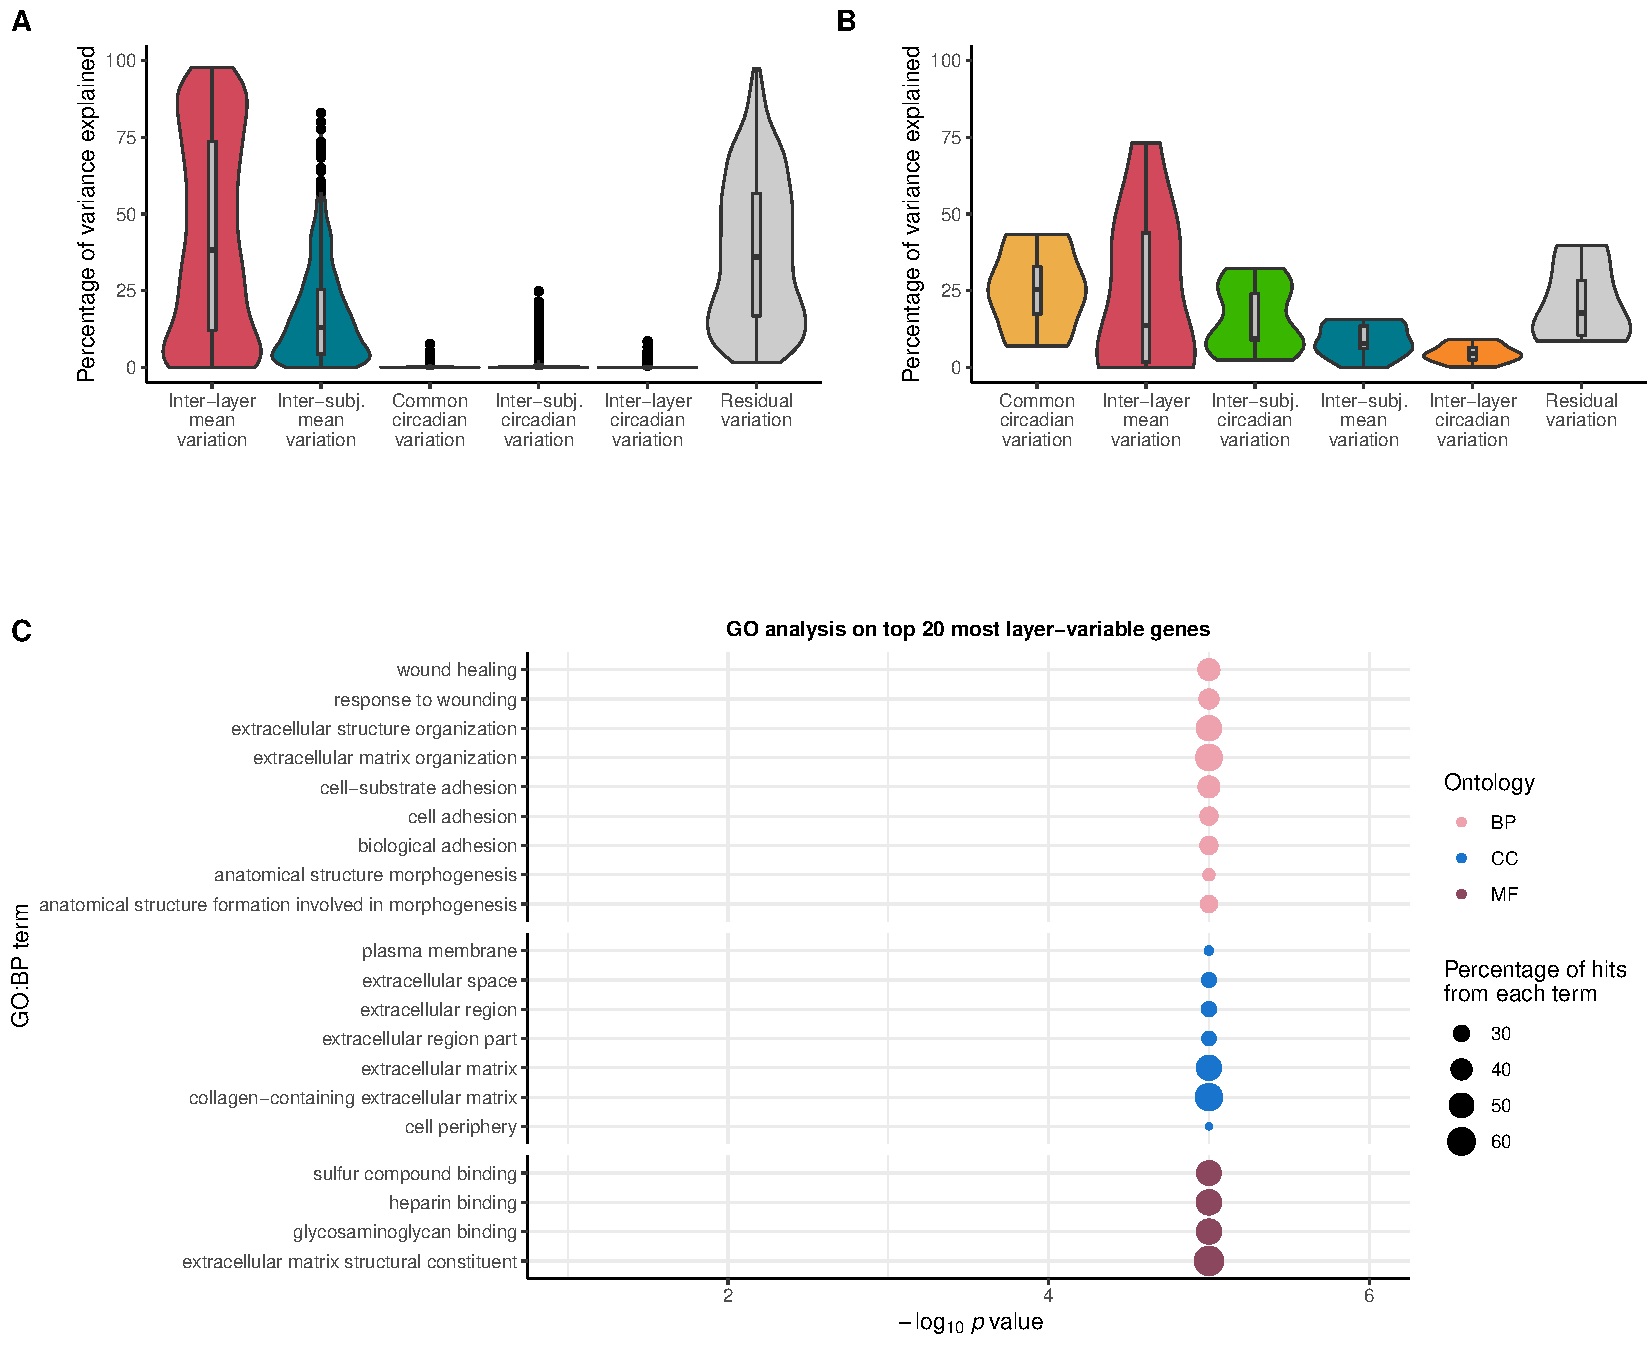
\includegraphics[scale=0.55]{./Figures/suppfig3_1.pdf}
		\caption{\textbf{Drivers of variation in the human skin circadian transcriptome. A.} Negative control of the \texttt{variancePartition} analysis: the pipeline was run in 1000 non-rhythmic genes (FDR$>$0.1) to show that external time does not represent a major source of variation among these transcripts. \textbf{B.} Positive control: \texttt{variancePartition} was run in the clock genes to show that time represents a major (in fact, the largest) source of variation.\textbf{ C.} GO enrichment analysis in the 200 circadian transcripts with largest variability in mean expression across layers. \textbf{D.} GO enrichment analysis in the 200 rhythmic transcripts with largest rhythm variability across layers, i.e., transcripts that show differential rhythms in human dermis versus epidermis. \textbf{E.} GO enrichment analysis in the 200 circadian transcripts with largest residual variability in mean expression. For C-E: the top 20 enriched terms (with a minimum gene set of 5 terms from each category) are shown; pink represents biological processes; blue, cellular compartment; purple, molecular function; enrichment was performed testing against the background of $\sim$1400 rhythmic genes in at least one layer.} %	Variance partition with external time. Positive and negative control + go analysis of top 200 most changing genes from categories of interest. background of go analyses are all rhythmic genes in D or E. GO with clusterProfiler, mingene set size=5}
		\label{fig:suppfig3}
	\end{center}
\end{figure*}
\clearpage

\begin{figure*}[h!tb]
	\begin{center}
		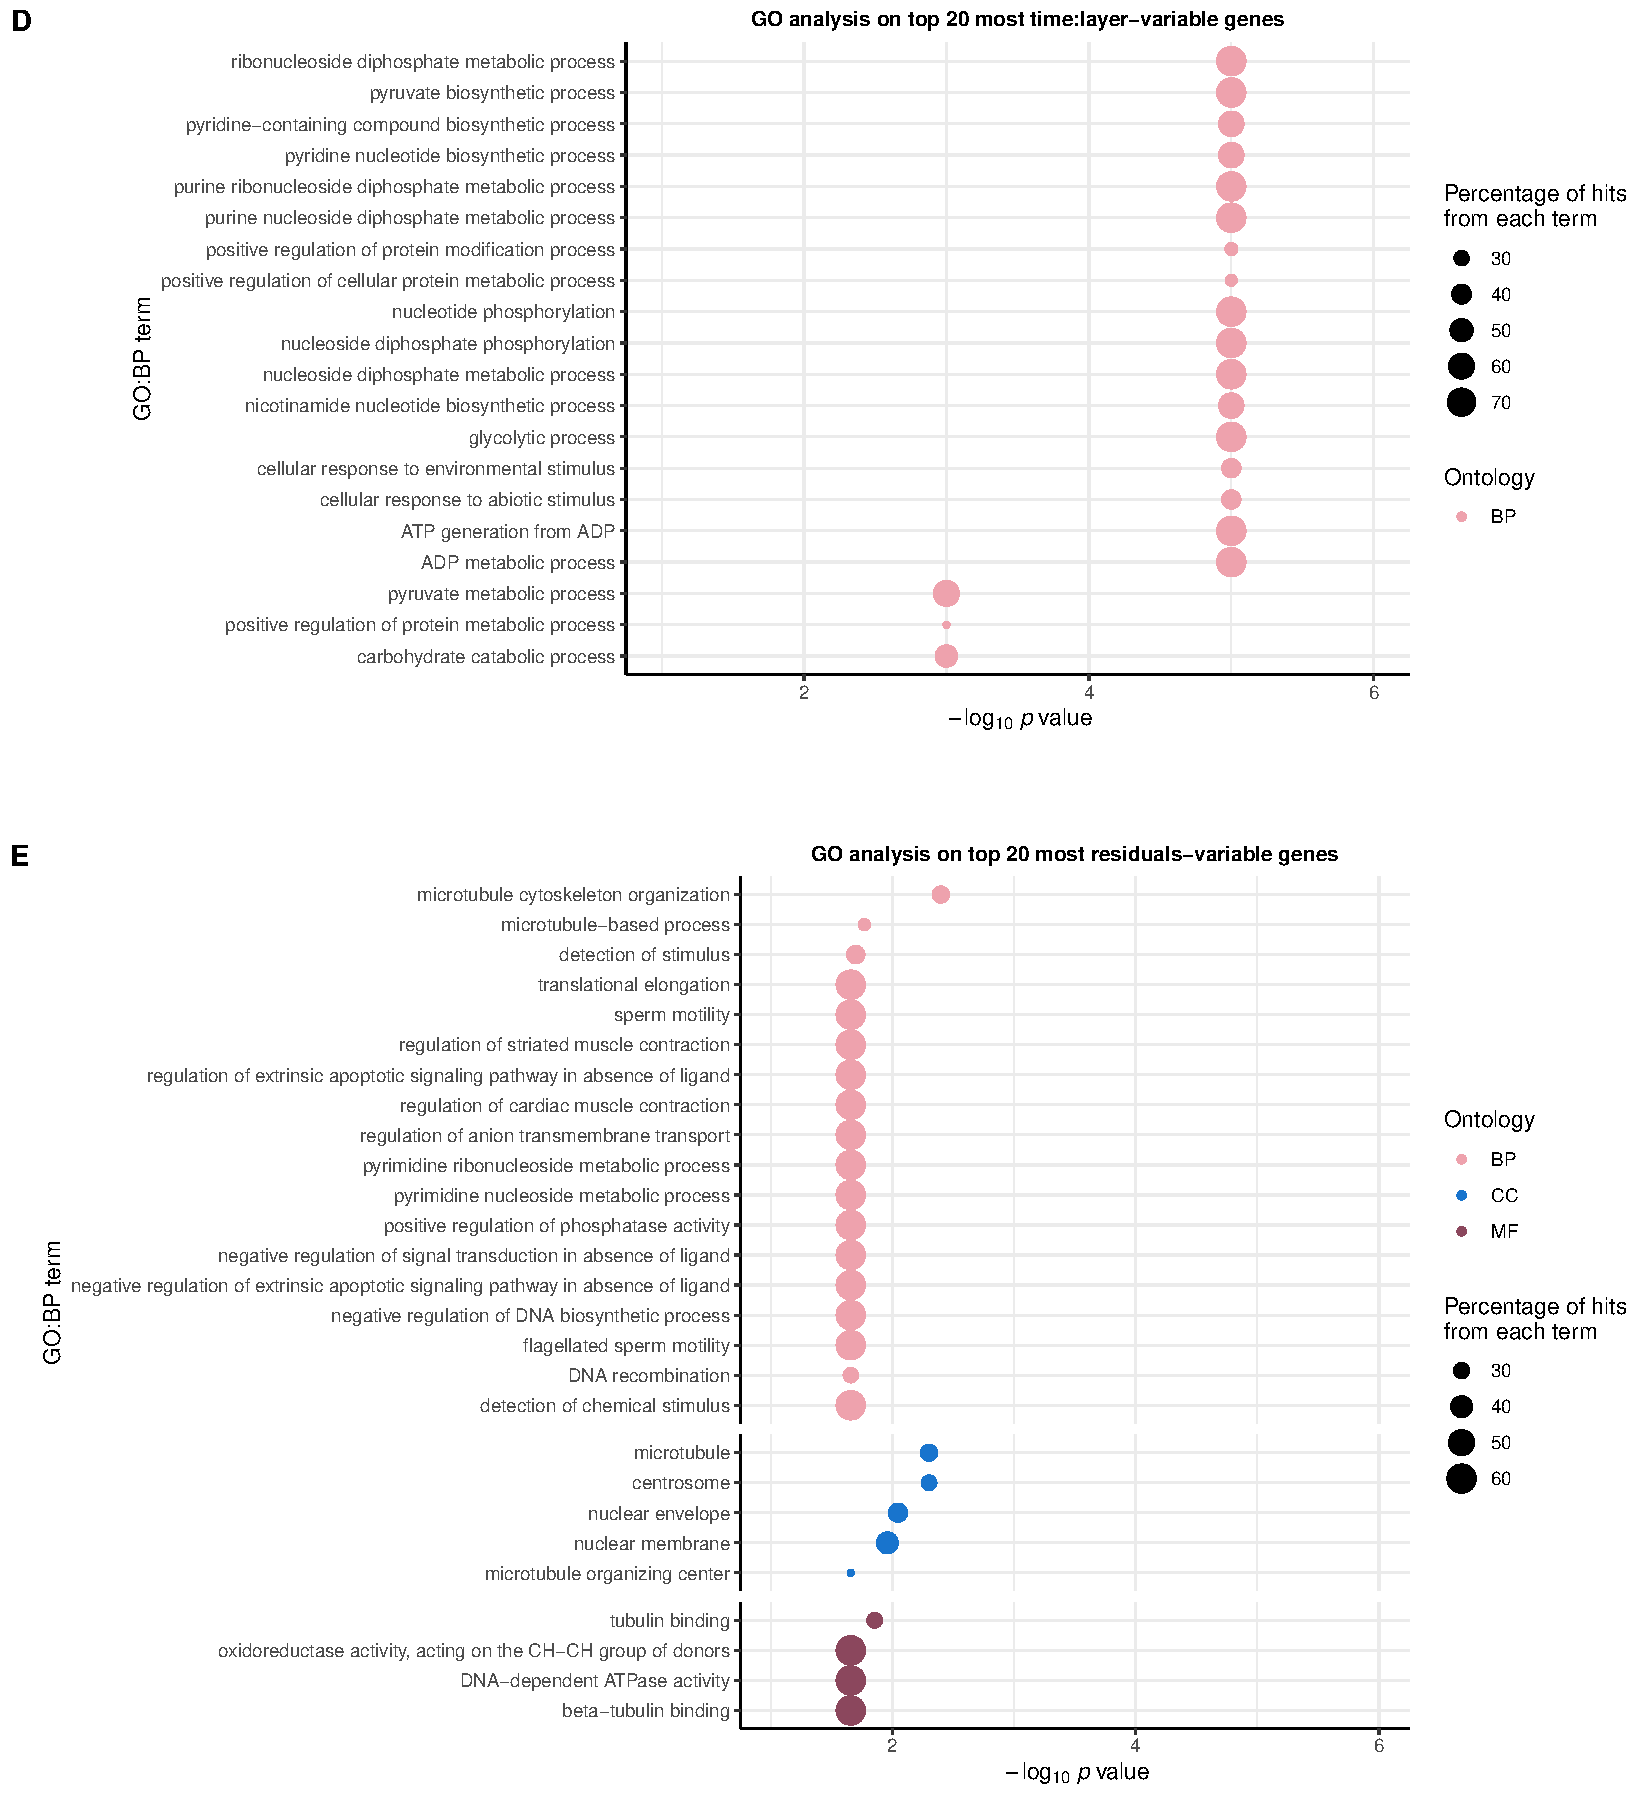
\includegraphics[scale=0.55]{./Figures/suppfig3_2.pdf}
		%\caption*{Suppfig3 continuation}
		%\label{fig:suppfig2}
	\end{center}
\end{figure*}
\clearpage


%----------------------------------------------------------------------------------------
%----------------------------------------------------------------------------------------

\begin{figure*}[h!tb]
	\begin{center}
		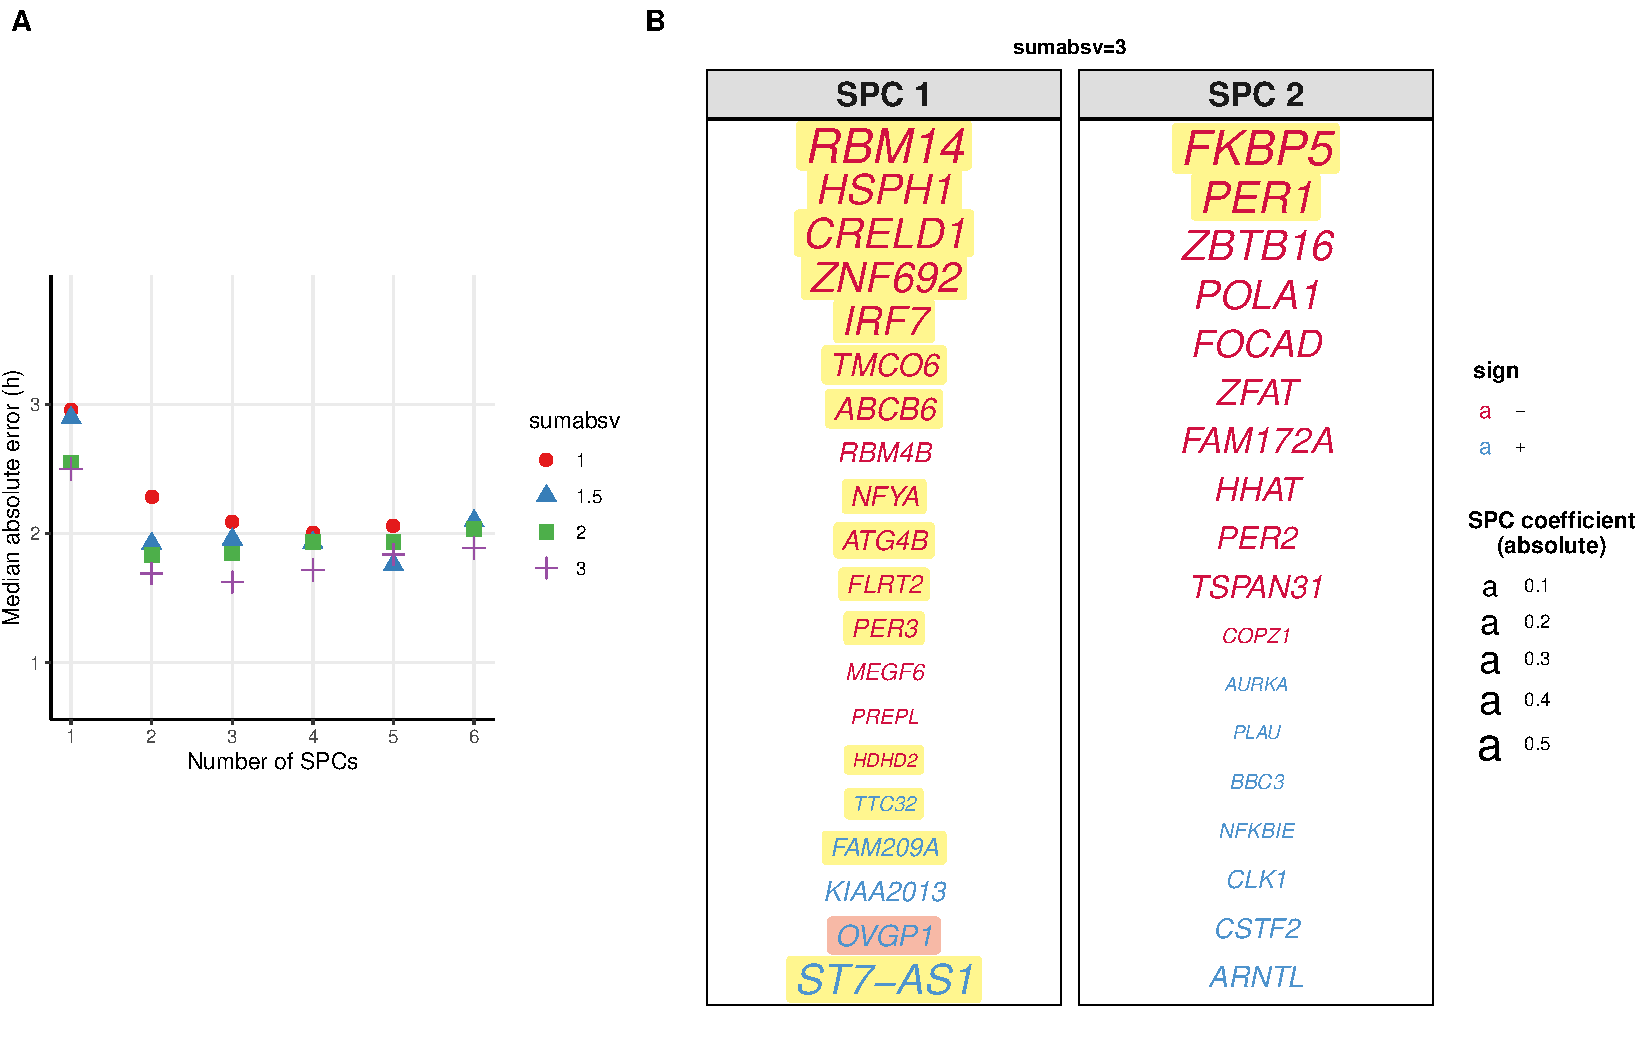
\includegraphics[scale=0.55]{./Figures/suppfig4.pdf}
		\caption{\textbf{Identification of internal time-telling genes in human skin with \texttt{ZeitZeiger} \cite{Hughey2016}. A.} Median absolute error of the internal-time prediction on cross-validation (see Materials and Methods for details) as a function of the two main parameters of \texttt{ZeitZeiger}, \texttt{sumabsv} and \texttt{nSPC}. \textbf{B. }Internal time predictors from human skin for \texttt{sumabsv}=3 and \texttt{nSPC}=2. Genes assigned to SPC1 or SPC2 as well as their coefficients are shown. Highlighted in yellow are genes that appeared in the top 20 most common circadian varying genes in the \texttt{variancePartition }analysis done in the rhythmic genes in human skin (i.e., in \textit{at least} one layer); in orange, genes that showed differential rhythms across layers (i.e., genes with high inter-layer circadian variation from the \texttt{variancePartition} analysis). Note, that the difference to Figure \ref{fig:fig3} is that here, \texttt{ZeitZeiger} was run once using the whole $\sim$11000 expressed genes in at least one layer, and not separately in each layer.}%ZeitZeiger with internal time in skin as a whole -- worse MAE
		\label{fig:suppfig4}
	\end{center}
\end{figure*}
\clearpage

%----------------------------------------------------------------------------------------
%----------------------------------------------------------------------------------------

\begin{figure*}[h!tb]
	\begin{center}
		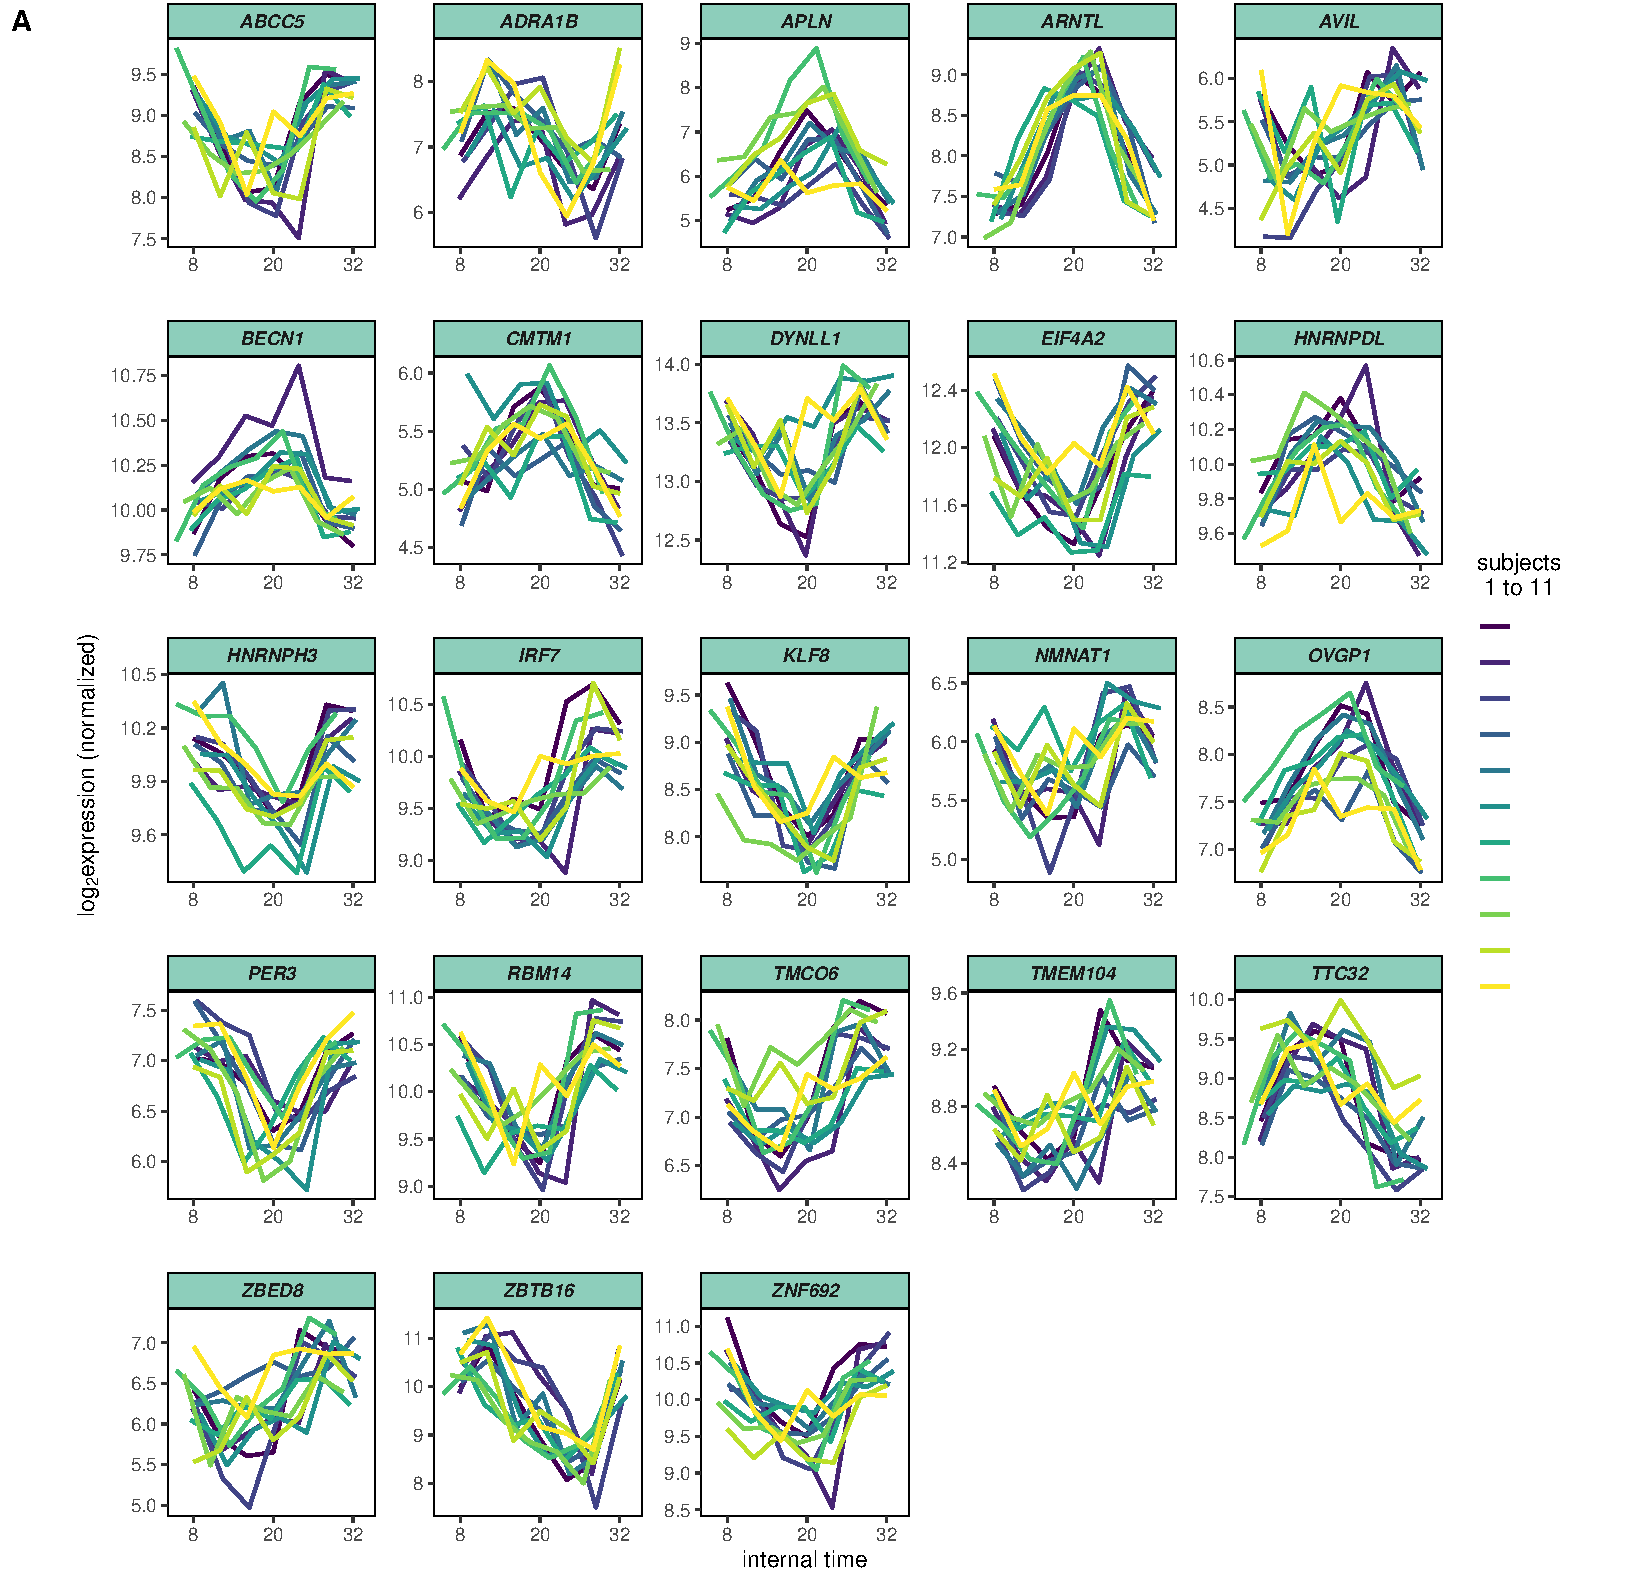
\includegraphics[scale=0.55]{./Figures/suppfig5_1.pdf}
		\caption{\textbf{Identification of internal time-telling genes in human dermis and epidermis with \texttt{ZeitZeiger} \cite{Hughey2016}. A. }Time series of expression of the time-telling genes in dermis (green) and epidermis (orange). Colored lines represent the expression profiles in different subjects. \textbf{B.} \texttt{variancePartition} analysis on the \texttt{ZeitZeiger} genes in dermis (left) or epidermis (right) shows high temporal variation and minor variability in mean expression across subjects. \textbf{C.} Expression profiles of the time-telling genes from our cohort in dermis (left) and epidermis (right) represented in SPC space and faceted by subject. Colors indicate internal time. \texttt{ZeitZeiger} was run with all $\sim11000$ expressed genes and separately for dermis and epidermis.}%ZeitZeiger in D and E separately with internal time. A) Timeseries of dermal ZZ genes
		\label{fig:suppfig5}
	\end{center}
\end{figure*}
\clearpage

\begin{figure*}[h!tb]
	\begin{center}
		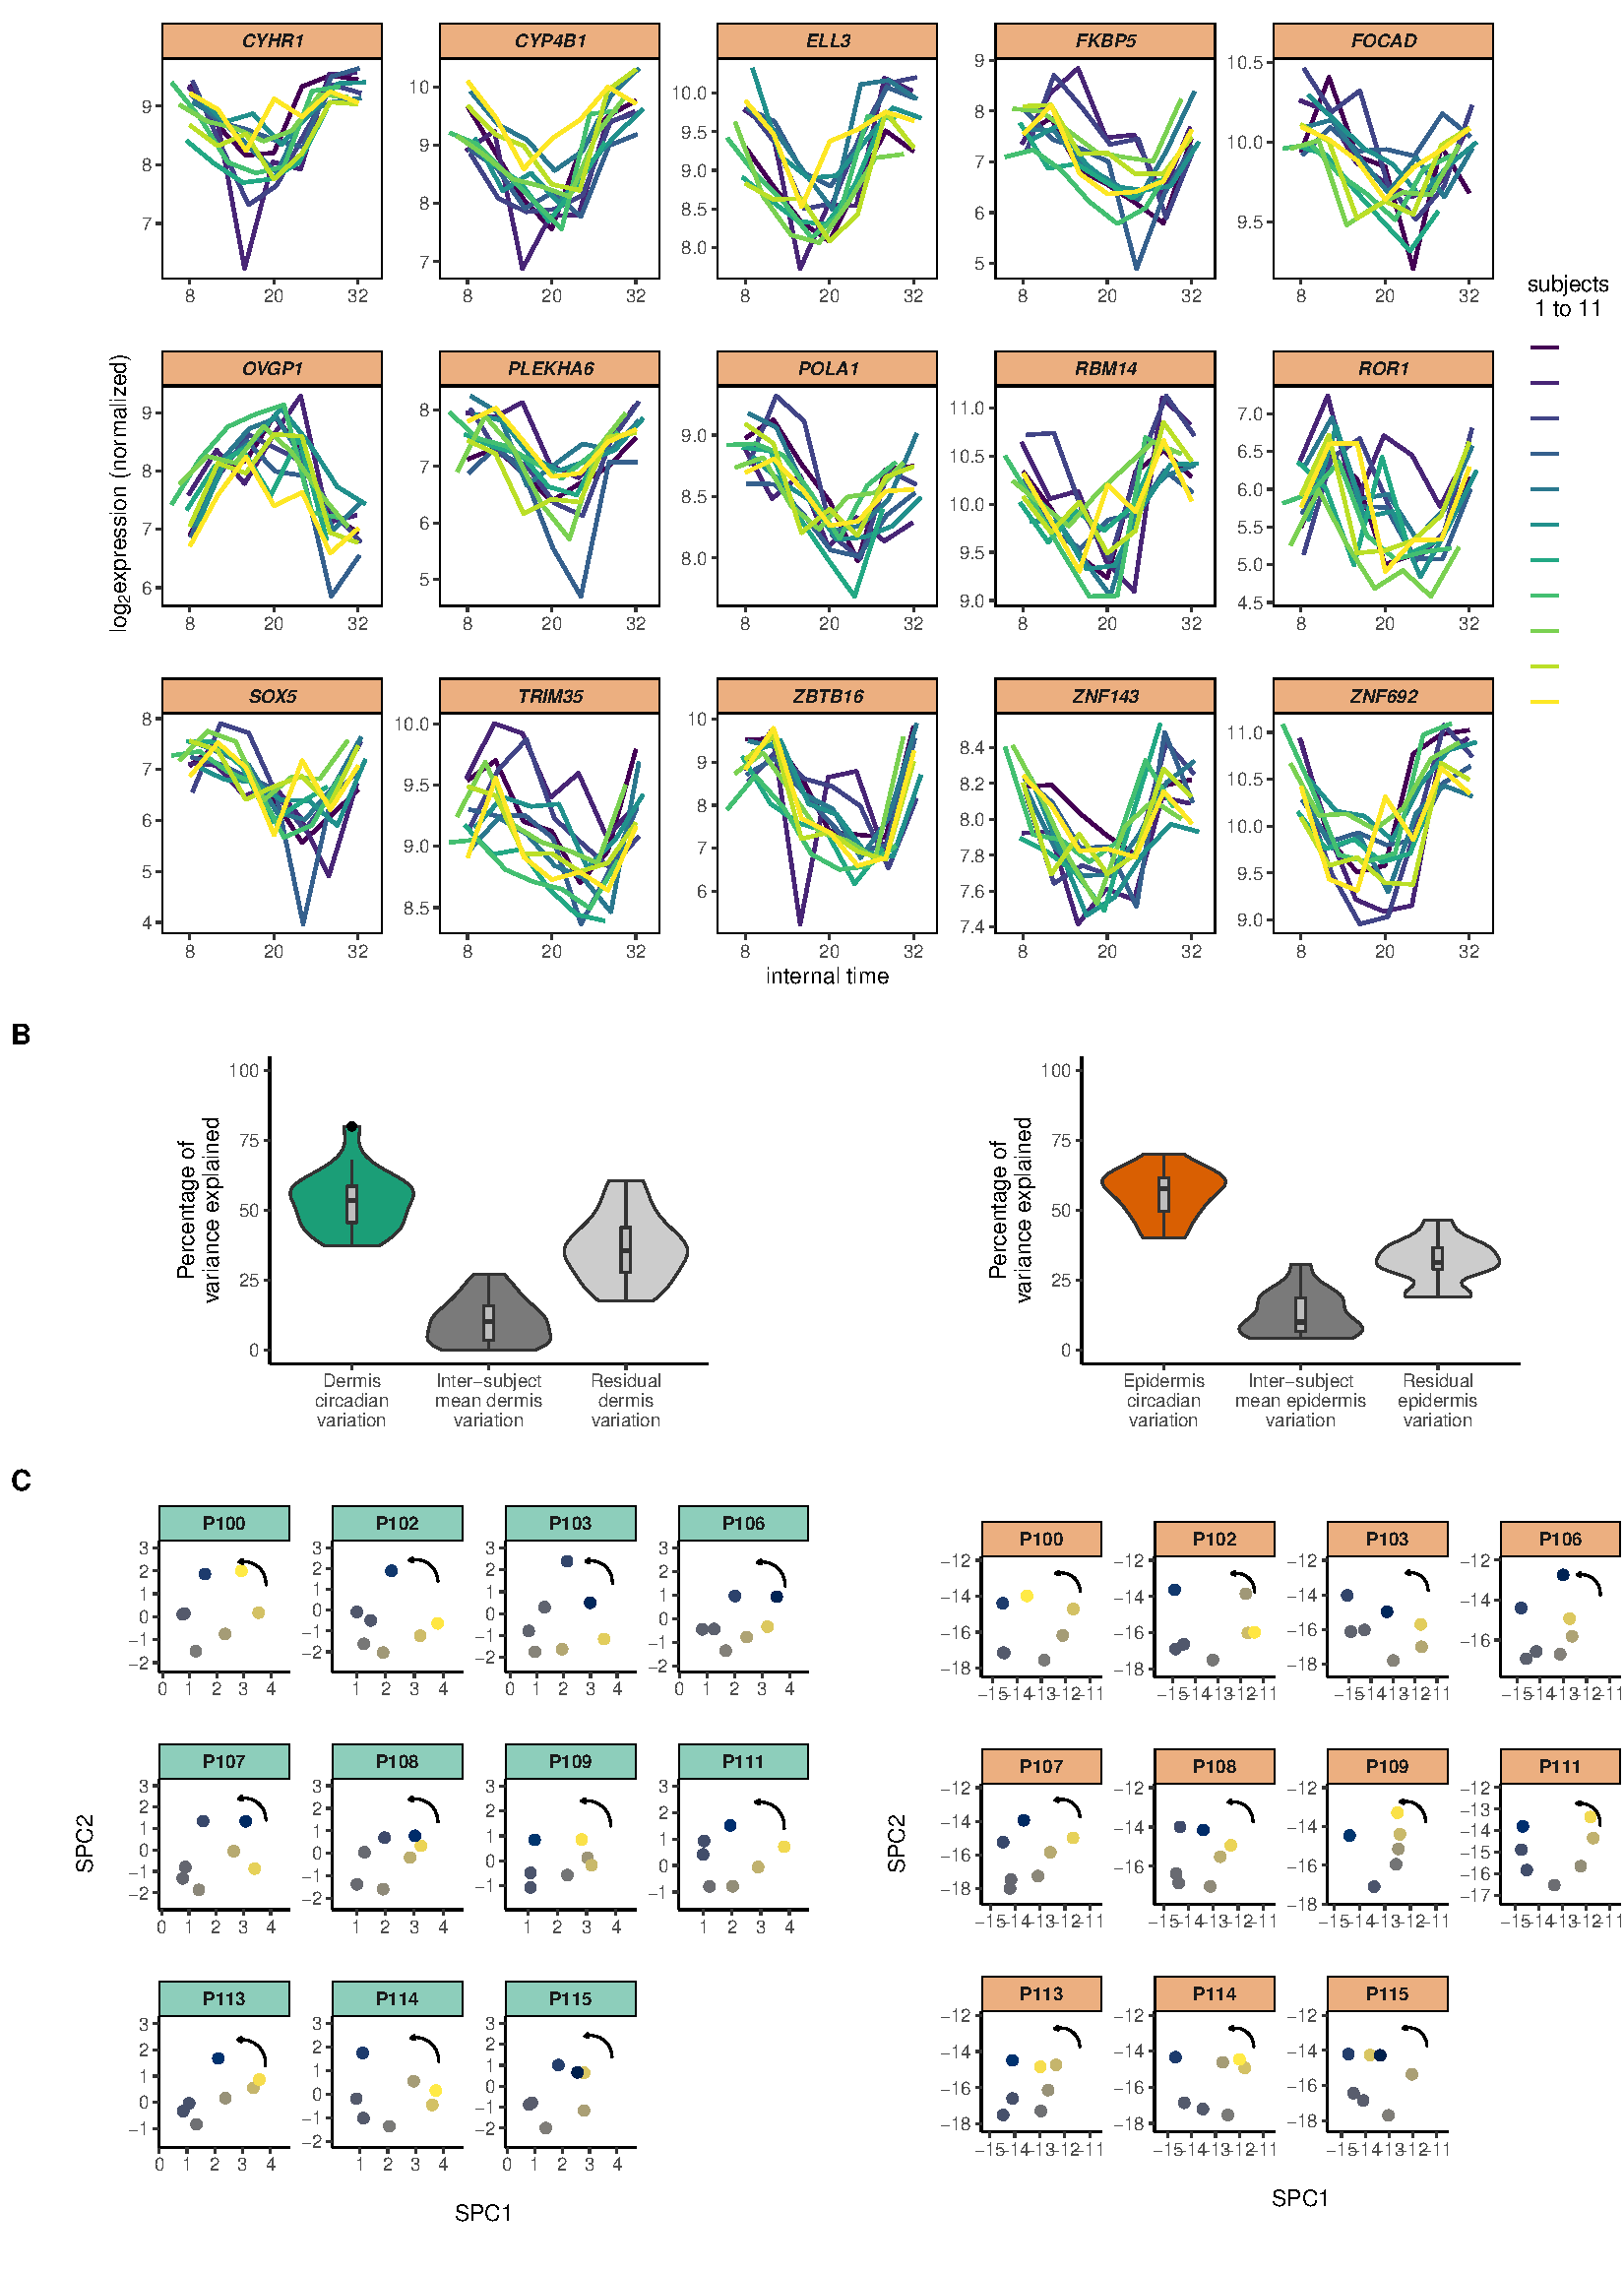
\includegraphics[scale=0.55]{./Figures/suppfig5_2.pdf}
		%\caption*{Continuation of Suppfig5. ZeitZeiger in D and E separately with internal time. A) Timeseries of epidermal ZZ genes}
		%\label{fig:suppfig2}
	\end{center}
\end{figure*}
\clearpage


%----------------------------------------------------------------------------------------
%----------------------------------------------------------------------------------------

\begin{table}[h!tb]\vspace{-.4cm}
	\caption{\textbf{Meta-data about the subjects collected for this study.} Mid sleep time was calculated and was corrected for the sleep-debt accumulated during the working days as described in \cite{Roenneberg2007, Vetter2021}.}
	\footnotesize \vspace{-.2cm}
	\begin{tabular}{ccccccccc}
		\hline
		\textbf{Subject} &
		\textbf{Sex} &
		\textbf{\begin{tabular}[c]{@{}c@{}}Birth\\year\end{tabular}} &
		\textbf{\begin{tabular}[c]{@{}c@{}}Bed time\\work days\end{tabular}} &
		\textbf{\begin{tabular}[c]{@{}c@{}}Sleep time\\work days\end{tabular}} &
		\textbf{\begin{tabular}[c]{@{}c@{}}Min\\fall asleep\\work days\end{tabular}} &
		\textbf{\begin{tabular}[c]{@{}c@{}}Wake up time\\work days\end{tabular}} &
		\textbf{\begin{tabular}[c]{@{}c@{}}Min\\wake up\\work days\end{tabular}} &
		\textbf{\begin{tabular}[c]{@{}c@{}}Alarm\\work days?\end{tabular}} \\ \hline
		P108 & male   & 1984 & 22:45 & 23:00 & 20  & 6:30 & 15 & Y  \\ 
		P100 & male   & 1991 & 23:00 & 23:00 & 7.5 & 7:00 & 5  & Y  \\
		P113 & male   & 1985 & 23:30 & 0:00  & 30  & 8:30 & 10 & Y  \\ 
		P106 & male   & 1982 & 23:00 & 23:15 & 15  & 6:52 & 7.5& Y  \\ 
		P102 & male   & 1989 & 23:00 & 23:00 & 10  & 7:30 & 0  & Y  \\ 
		P109 & male   & 1984 & 23:00 & 23:00 & 5   & 8:00 & 0  & Y  \\ 
		P103 & female & 1988 & 0:00  & 0:25  & 25  & 7:30 & 9  & Y  \\ 
		P107 & female & 1987 & 23:00 & 23:00 & 15  & 6:00 & 5  & Y  \\ 
		P111 & female & 1983 & 0:00  & 0:00  & 5   & 8:00 & 15 & Y  \\ 
		P114 & female & 1986 & 23:30 & 23:30 & 5   & 8:30 & 5  & Y  \\ 
		P115 & female & 1981 & 22:00 & 22:15 & 5   & 5:20 & 5  & Y  \\ \hline
	\end{tabular}\vspace{0.2cm}
	\begin{tabular}{cccccccc}
		\hline
		\textbf{Subject} &
		\textbf{\begin{tabular}[c]{@{}c@{}}Wake up\\before alarm?\end{tabular}} &
		\textbf{\begin{tabular}[c]{@{}c@{}}Bed time\\free days\end{tabular}} &
		\textbf{\begin{tabular}[c]{@{}c@{}}Sleep time\\free days\end{tabular}} &
		\textbf{\begin{tabular}[c]{@{}c@{}}Min\\fall asleep\\free days\end{tabular}} &
		\textbf{\begin{tabular}[c]{@{}c@{}}Wake up time\\free days\end{tabular}} &
		\textbf{\begin{tabular}[c]{@{}c@{}}Wake up time\\free days\end{tabular}} &
		\textbf{\begin{tabular}[c]{@{}c@{}}Alarm\\free days?\end{tabular}} \\ \hline
		P108 & Y & 23:00 & 23:15 & 15 & 6:30  & 30 & N \\ 
		P100 & N & 0:00  & 0:00  & 5  & 8:00  & 15 & Y \\
		P113 & N & 1:00  & 1:15  & 20 & 9:30  & 15 & Y \\ 
		P106 & Y & 23:30 & 23:45 & 15 & 9:15  & 60 & Y \\ 
		P102 & N & 0:00  & 0:00  & 10 & 8:00  & 10 & N \\ 
		P109 & Y & 0:00  & 0:00  & 5  & 8:30  & 30 & N \\ 
		P103 & N & 0:00  & 0:00  & 25 & 7:30  & 5  & Y \\ 
		P107 & Y & 0:00  & 0:00  & 15 & 7:30  & 5  & N \\ 
		P111 & Y & 2:30  & 2:30  & 5  & 11:00 & 30 & N \\ 
		P114 &   & 23:30 & 23:30 & 5  & 8:30  & 5  & N \\ 
		P115 & N & 0:00  & 0:15  & 5  & 8:30  & 30 & N \\ \hline
	\end{tabular}\vspace{0.2cm}
	\begin{tabular}{cc}
		\hline
		\textbf{Subject} & \textbf{\begin{tabular}[c]{@{}c@{}}Corrected\\mid sleep time\end{tabular}} \\ \hline
		P108             & 02:58           \\
		P100             & 04:00           \\
		P113             & 05:28           \\
		P106             & 03:50           \\
		P102             & 04:11           \\
		P109             & 04:26           \\
		P103             & 03:36           \\
		P107             & 03:34           \\
		P111             & 06:34           \\
		P114             & 04:00           \\
		P115             & 03:58          \\ \hline
	\end{tabular}	
	\label{tab:supptab1}
\end{table}

%----------------------------------------------------------------------------------------
%----------------------------------------------------------------------------------------

%https://genomemedicine.biomedcentral.com/articles/10.1186/s13073-020-00768-9#Sec19
%\begin{table}[b!ht]\vspace{-.3cm}
%	\caption{\textbf{List of software packages used in this study.} Versions and references are included. }\vspace{-.2cm}
%	\footnotesize
%	\centering
%\begin{tabular}{llc}
%	\hline
%	\textbf{\begin{tabular}[c]{@{}c@{}}Software\\package\end{tabular}} & \textbf{Version} & \textbf{Ref.}     \\ \hline
%	Biobase                   & 2.46.0           & \cite{biobase}         \\
%	clusterProfiler           & 3.14.3           & \cite{clusterprofiler} \\
%	cowplot                   & 1.1.1            & \cite{cowplot}         \\
%	doParallel                & 1.0.16           & \cite{doparallel}      \\
%	dplyr                     & 1.0.5            & \cite{dplyr}           \\
%	GEOquery                  & 2.54.1           & \cite{geoquery}        \\
%	ggforce                   & 0.3.3            & \cite{ggforce}         \\
%	ggplot2                   & 3.3.3            & \cite{ggplot2}         \\
%	ggrepel                   & 0.9.1            & \cite{ggrepel}         \\
%	ggthemes                  & 4.2.4            & \cite{ggthemes}        \\ \hline
%\end{tabular}	
%\hspace{0.2cm}
%\begin{tabular}{llc}
%	\hline
%	\textbf{\begin{tabular}[c]{@{}c@{}}Software\\package\end{tabular}} & \textbf{Version} & \textbf{Ref.}     \\ \hline
%	ggvenn                    & 0.1.8            & \cite{ggvenn}          \\
%	hgug4112a.db              & 3.2.3            & \cite{hgug4112a}       \\
%	hms                       & 1.0.0            & \cite{hms}             \\
%	limma                     & 3.42.2           & \cite{limma}           \\
%	lubridate                 & 1.7.10           & \cite{lubridate}       \\
%	magrittr                  & 2.0.1            & \cite{magrittr}        \\
%	msigdbr                   & 7.4.1            & \cite{msigdbr}         \\
%	\textcolor{red}{oligo??}  &                  & \textbf{which?}        \\
%	PSEA                      & 1.1              & \cite{Zhang2016}       \\
%	R                         & 3.6.3            & \cite{R}               \\ \hline
%\end{tabular}
%\hspace{0.2cm}	
%\begin{tabular}{llc}
%	\hline
%	\textbf{\begin{tabular}[c]{@{}c@{}}Software\\package\end{tabular}} & \textbf{Version} & \textbf{Ref.}     \\ \hline
%	stringr                   & 1.4.0            & \cite{stringr}         \\
%	tibble                    & 3.1.1            & \cite{tibble}          \\
%	tidyr                     & 1.1.3            & \cite{tidyr}           \\
%	tidytext                  & 0.3.2            & \cite{tidytext}        \\
%	tidyverse                 & 1.3.1            & \cite{tidyverse}       \\
%	variancePartition         & 1.16.1           & \cite{Hoffman2016}     \\
%	viridis                   & 0.6.1            & \cite{viridis}         \\
%	zeitzeiger                & 2.0.2            & \cite{Hughey2016}      \\ 
%	                          &                  &                        \\
%	                          &                  &                        \\ \hline
%\end{tabular}	
%	\label{tab:supptab2}

%\end{table}
\clearpage
